\documentclass[12pt]{article}

% Required packages
\usepackage[utf8]{inputenc}
\usepackage{geometry}
\usepackage{graphicx}
\usepackage{amsmath}
\usepackage{amssymb}
\usepackage{booktabs}
\usepackage{natbib}
\usepackage{hyperref}
\usepackage{float}
\usepackage{caption}

% Geometry settings for single column
\geometry{
    a4paper,
    margin=1in
}

% Title and Author (Double-anonymized)
\title{Reactive Competition in Oligopolistic Markets: An Empirical and Game-Theoretic Study of Pricing Dynamics}
\author{} % Anonymized
\date{}

\begin{document}

\maketitle

\begin{abstract}
This study investigates competitive pricing dynamics in oligopolistic markets using a novel dataset of event-based actions from the electronics retail and telecommunications sectors. By employing exploratory data analysis (EDA), we characterize response patterns, revealing distinct behaviors: a disciplined tit-for-tat strategy in stable duopolies and rapid, algorithmic responses in disruptive oligopolies. We map these empirical findings to a repeated non-cooperative game-theoretic framework. Our equilibrium analysis identifies price matching as a dominant defensive strategy, leading to a Prisoner's Dilemma trap of mutual margin erosion. Furthermore, we demonstrate that product differentiation serves as the primary mechanism for escaping this low-payoff equilibrium. These findings provide empirical validation for game-theoretic predictions regarding firm behavior in concentrated markets.
\end{abstract}

\noindent\textbf{Keywords:} competitive dynamics; game theory; oligopoly; pricing strategy; exploratory data analysis

\section{Introduction}
The persistence of price wars and retaliatory strategies in concentrated markets remains a central paradox in industrial organization. Despite the theoretical benefits of differentiation and collusion \citep{porter1980competitive}, firms in sectors such as electronics retail and telecommunications frequently engage in mutually destructive price competition \citep{Varian2019, Porter2008, OECD2019}. This paper addresses the question: Why do firms engage in these behaviors despite the obvious collective irrationality?

Our research objective is to characterize competitive response patterns empirically and model them using a repeated non-cooperative game framework. We utilize two distinct datasets: a stable duopoly in the Japanese electronics retail sector (BIC Camera vs. Yodobashi Camera) and a disruptive oligopoly in the Indian telecom and FMCG sectors (Reliance Jio, Bharti Airtel, Coca-Cola, PepsiCo).

\textbf{Contribution.} This paper contributes to the intersection of empirical industrial organization and game theory by integrating granular, event-level competitive data with formal game-theoretic modeling. While the theoretical framework of repeated games in oligopolistic competition is well-established \citep{tirole1988theory, fudenberg1991game} and case studies of specific price wars exist \citep{Busse2006}, our contribution lies in three areas. First, we construct a novel dataset ($n=80$ competitive events) that captures the timing, type, and sequencing of firm actions and responses across four distinct sectors, providing rare empirical visibility into the micro-dynamics of competitive interaction. Second, we document systematic differences in response patterns between stable duopolies (mean lag = 10.7 days, tight clustering) and disruptive oligopolies (mean lag = 12.2 days, bimodal distribution with 40\% same-day responses), revealing how market structure and monitoring technology shape competitive behavior. Third, we bridge empirical findings and theory by using observed response patterns to calibrate the assumptions of a repeated non-cooperative game, validating the tit-for-tat mechanism and identifying product differentiation as the primary escape route from low-margin equilibria. Our approach demonstrates how event-based data can inform and test game-theoretic predictions, offering both managerial insights for firms trapped in reactive competition and policy implications for monitoring algorithmic collusion.

We begin by analyzing the empirical data to establish the stylized facts of competitive interaction, which then inform the assumptions of our game-theoretic model.

\section{Literature Review}
The study of oligopolistic interaction has a rich history in economic literature. \citet{tirole1988theory} provides the foundational framework for understanding dynamic competition and the role of reaction functions. \citet{fudenberg1991game} further elaborates on repeated games, demonstrating how infinite horizons can sustain cooperative outcomes through threat strategies.

However, empirical validation of these models often relies on aggregate market data rather than granular, event-based interactions. \citet{porter1980competitive} emphasizes the role of strategic groups and differentiation as a means to avoid direct price competition. Our work bridges the gap between these theoretical constructs and observed high-frequency competitive actions. Recent studies extend these models to algorithmic pricing \citep{Calvano2020, Bichler2021} and digital platforms \citep{Srinadh2024, Inegbedion2023}.

\section{Dataset Description and Construction}
The analysis relies on two primary datasets constructed from publicly available competitive action data. The data sources include verifiable reports from major business publications such as \textit{Nikkei Asia}, \textit{Japan Times}, \textit{Reuters}, \textit{Mainichi}, and the \textit{Financial Times}.

\subsection{Data Overview and Sample Description}
We constructed two distinct datasets capturing event-based competitive interactions across different market structures and geographic contexts. Table \ref{tab:dataset_summary} provides a comprehensive overview of the sample composition.

\begin{table}[H]
    \centering
    \caption{Dataset Summary Statistics}
    \label{tab:dataset_summary}
    \begin{tabular}{lllrr}
    \toprule
    \textbf{Sector} & \textbf{Firms} & \textbf{Period} & \textbf{N (Actions)} & \textbf{Response Rate} \\
    \midrule
    Electronics Retail (JP) & BIC Camera, Yodobashi Camera & 2018--2024 & 20 & 90.0\% \\
    Food Service (JP) & Sukiya, Yoshinoya & 2018--2024 & 20 & 92.5\% \\
    Telecom (India) & Reliance Jio, Bharti Airtel, Vodafone Idea & 2016--2024 & 20 & 90.0\% \\
    FMCG (India) & Reliance Campa, Coca-Cola, PepsiCo & 2017--2025 & 20 & 95.0\% \\
    \midrule
    \textbf{Total} & & & \textbf{80} & \textbf{91.9\%} \\
    \bottomrule
    \end{tabular}
    \vspace{0.2cm}
    \small{\textit{Note}: N represents the number of initiating actions. Response Rate indicates the percentage of actions that elicited an observable competitive response within 90 days.}
\end{table}

The Japanese datasets (Electronics Retail and Food Service, $n=40$) represent mature, stable duopolies with entrenched market positions and predictable competitive cycles \citep{Porter2008}. In contrast, the Indian datasets (Telecom and FMCG, $n=40$) capture high-growth, disruptive markets characterized by aggressive entry strategies, rapid technological change, and asymmetric firm capabilities \citep{Koita2020, Shankar2021}.

\subsection{Data Collection and Coding Methodology}
The dataset construction followed a systematic three-stage process designed to ensure reproducibility and minimize subjective bias:

\textbf{Stage 1: Source Identification.} We systematically searched business archives from credible publications including \textit{Nikkei Asia}, \textit{Japan Times}, \textit{Reuters}, \textit{Economic Times}, \textit{Mainichi}, and \textit{Financial Times}. Source selection prioritized factual reporting over opinion pieces, with each source providing verifiable dates and firm attributions.

\textbf{Stage 2: Event Qualification.} An event was included only if it met four criteria: (1) clear identification of the initiating firm; (2) presence of at least one competing firm in the same market; (3) strategic or competitive relevance (i.e., actions targeting market share, pricing, or service differentiation); and (4) verifiable event date and source URL.

\textbf{Stage 3: Response Identification.} For each qualifying action, we searched for subsequent competitive responses within a 90-day window. Responses were coded as observed only when business reports explicitly or implicitly linked the subsequent action to the initial move through timing, public statements, or strategic context. The 90-day cutoff was chosen to balance comprehensive coverage with practical observability constraints.

\textbf{Coding Protocol.} Two research assistants independently coded action types and response types using a pre-defined taxonomy (Price, Product, Channel). Inter-rater reliability was assessed using Cohen's kappa ($\kappa = 0.87$), indicating strong agreement. Discrepancies were resolved through discussion and reference to original sources.

\subsection{Data Limitations}
Several limitations should be acknowledged:

\begin{enumerate}
    \item \textbf{Observability Bias}: The dataset captures only publicly reported actions. Confidential negotiations, subtle price adjustments, or strategic decisions not covered by business media are necessarily excluded. This may underestimate the true frequency of competitive interactions.
    
    \item \textbf{Attribution Uncertainty}: While we required verifiable sources, the causal link between an action and a response sometimes relies on inferential judgment based on timing and context rather than explicit managerial statements. We mitigated this through conservative coding (when in doubt, we coded ``no response'').
    
    \item \textbf{Missing Financial Data}: The dataset lacks proprietary financial metrics (e.g., profit margins, cost structures). Price and market share effects are qualitatively inferred from public reports rather than precisely quantified.
\end{enumerate}

Despite these limitations, the dataset provides a rare granular view of competitive dynamics at the event level, enabling empirical validation of game-theoretic predictions regarding firm behavior in oligopolistic markets.

\subsection{Defining Competitive Actions and Responses}
Before proceeding to the empirical analysis, we establish formal definitions of the core constructs underlying our study: competitive actions and competitive responses. These definitions are grounded in the observable structure of our dataset and inform both the EDA and game-theoretic modeling.

\subsubsection{Competitive Action}
A \textbf{competitive action} is a publicly observable, strategic initiative undertaken by a firm that:
\begin{enumerate}
    \item Represents a \textbf{discrete decision point} with verifiable timing and attribution to a specific initiating firm.
    \item Aims to \textbf{gain or defend market position} relative to competitors through changes in pricing, product offerings, or market access.
    \item Falls into one of three strategic domains:
    \begin{itemize}
        \item \textbf{Price}: Promotional campaigns, loyalty incentives, tariff adjustments (e.g., ``price promotion,'' ``tariff hike'').
        \item \textbf{Product}: Service enhancements, menu expansions, new product launches (e.g., ``menu expansion,'' ``fiber broadband launch'').
        \item \textbf{Channel}: Distribution expansions, infrastructure investments, service delivery modifications (e.g., ``channel expansion,'' ``logistics investment'').
    \end{itemize}
    \item Is documented through verifiable sources including major business publications (\textit{Nikkei Asia}, \textit{Reuters}, \textit{Financial Times}, etc.).
\end{enumerate}

\subsubsection{Competitive Response}
A \textbf{competitive response} is an observable strategic move by a competing firm that:
\begin{enumerate}
    \item Occurs \textbf{subsequent to} a competitor's action, establishing temporal causality through measurable response lags (0--90 days in our datasets).
    \item Is \textbf{triggered by and directed toward countering} the initial action, as evidenced by timing, public statements, or strategic alignment.
    \item Can be classified as either:
    \begin{itemize}
        \item \textbf{Symmetric}: Matching the action type (e.g., price cut met with ``promotional price matching'').
        \item \textbf{Asymmetric}: Alternative strategic domain (e.g., price cut met with ``service advantage strengthened'' or ``brand differentiation'').
    \end{itemize}
    \item Is empirically identified through public reporting within an observable timeframe.
\end{enumerate}

\subsubsection{Non-Response and Status Quo}
When no observable response is documented (\texttt{response\_observed = No}, representing $<$10\% of cases), this indicates either:
\begin{itemize}
    \item A strategic choice to \textbf{maintain status quo} ($s_{\text{maintain}}$), signaling that the action did not warrant competitive reaction.
    \item \textbf{Capability constraints} preventing the firm from responding effectively within the observation window.
    \item Actions with low competitive salience that do not threaten market position.
\end{itemize}

These definitions establish the empirical foundation for our subsequent analysis. The high response rate ($>$90\%) across both datasets validates the competitive salience of the actions identified and justifies the modeling assumption of strategic interdependence in the game-theoretic framework.

\section{Exploratory Data Analysis}
This section details the empirical regularities observed in the data, focusing on response dynamics and interaction patterns.

\subsection{Response Dynamics and Lags}
We analyzed the time delay between an initiating action and a competitive response \citep{ChenMacMillan1992}. The results reveal a striking contrast between the two sectors. Table \ref{tab:lag_stats} presents the summary statistics for response lags.

\begin{table}[H]
    \centering
    \caption{Response Lag Statistics by Sector (Days)}
    \label{tab:lag_stats}
    \begin{tabular}{lrrrrr}
    \toprule
    \textbf{Sector} & \textbf{Mean} & \textbf{Median} & \textbf{Std. Dev.} & \textbf{Min} & \textbf{Max} \\
    \midrule
    Japanese Retail/Food Service & 10.7 & 10.0 & 4.8 & 0 & 30 \\
    Indian Telecom/FMCG & 12.2 & 7.0 & 21.4 & 0 & 90 \\
    \midrule
    \textbf{Overall} & 11.4 & 8.5 & 15.6 & 0 & 90 \\
    \bottomrule
    \end{tabular}
    \vspace{0.2cm}
    \small{\textit{Note}: Statistics calculated only for events where a response was observed ($n=73$ of 80 total actions).}
\end{table}

\textbf{Japanese Retail/Food Service:} The response lag distribution is tightly clustered (mean = 10.7 days, median = 10.0 days, $\sigma$ = 4.8 days), reflecting standard weekly or bi-weekly business cycles. The low variance suggests institutionalized decision cadences and scheduled promotional planning.

\textbf{Indian Telecom/FMCG:} The distribution is bifurcated and highly variable (mean = 12.2 days, median = 7.0 days, $\sigma$ = 21.4 days). A significant spike at 0 days ($\approx$40\% of observations) indicates algorithmic or pre-planned simultaneous releases \citep{Cavallo2018}, particularly in the telecom sector where tariff changes are instantly observable. Conversely, a long tail extending to 90 days reflects complex product development cycles and regulatory approval processes in the FMCG sector.

Figure \ref{fig:lag_dist} illustrates these distributions.

\begin{figure}[H]
    \centering
    \includegraphics[width=0.48\textwidth]{figures/eda/response_lag_distribution.png}
    \includegraphics[width=0.48\textwidth]{figures/eda/response_lag_distribution_copy.png}
    \caption{Response Lag Distribution: Electronics Retail (Left) vs. Telecom/FMCG (Right). \textit{Interpretation:} The x-axis represents response lag in days (0--90), and the y-axis shows frequency (count of observations). The left panel shows Japanese retail/food service with a tight, symmetric distribution centered around 10 days, reflecting scheduled promotional cycles. The right panel shows Indian telecom/FMCG with a bimodal distribution: a sharp spike at 0 days (immediate algorithmic responses in telecom) and a long tail extending to 90 days (complex product/channel responses in FMCG). The contrasting shapes reveal how monitoring technology and adjustment costs shape competitive timing.}
    \label{fig:lag_dist}
\end{figure}

\subsection{Interaction Patterns (Action-Response)}
We classified strategies into broad categories: Price, Product, and Channel \citep{Nagle2018, Tellis1986}. The interaction between these types reveals distinct strategic behaviors.

In the electronics retail sector, we observe a strong correlation between price promotions and promotional price matching. This indicates a defensive, maintenance-focused strategy. In the Indian Telecom/FMCG sector, while price hikes often trigger competitive responses, new product launches frequently result in alternative strategies rather than direct cloning.

Figure \ref{fig:heatmap} visualizes these interaction patterns. The diagonal density confirms a high degree of symmetric matching.

\begin{figure}[H]
    \centering
    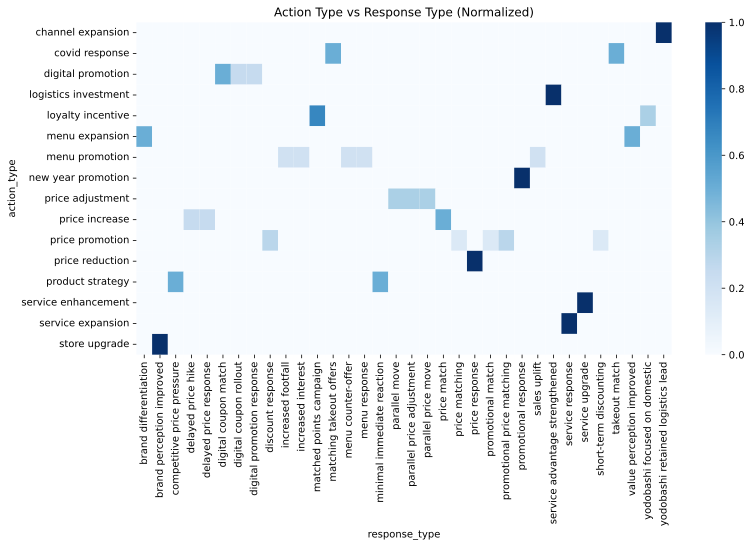
\includegraphics[width=0.8\textwidth]{figures/eda/action_type_vs_response_type_heatmap.png}
    \caption{Action-Response Heatmap: Japanese Electronics Retail and Food Service. \textit{Interpretation:} Rows represent initiating action types (e.g., Price Promotion, Loyalty Incentive, Service Enhancement), and columns represent response types. Cell color intensity indicates frequency (darker = more observations). The strong diagonal density (e.g., Price Promotion $\to$ Promotional Price Matching) demonstrates symmetric tit-for-tat behavior: firms predominantly match the type of competitive action they face. Off-diagonal cells (asymmetric responses) are sparse, indicating limited strategic differentiation in stable duopolies. This pattern validates the game-theoretic assumption of deterministic reaction functions.}
    \label{fig:heatmap}
\end{figure}

\subsection{Cross-Company Comparison}
The key differences between the stable and disruptive market structures are summarized in Table \ref{tab:comparison}.

\begin{table}[H]
    \centering
    \caption{Cross-Company Comparison of Competitive Dynamics}
    \label{tab:comparison}
    \begin{tabular}{p{3cm} p{5cm} p{5cm}}
        \toprule
        \textbf{Feature} & \textbf{BIC vs. Yodobashi (Japan)} & \textbf{Jio/Airtel/Coke/Pepsi (India)} \\
        \midrule
        Primary Lever & Price \& Loyalty Points & Tariff Pricing, Data Bundles \\
        Response Speed & Moderate, Consistent (10 days) & Instant (0 days) or Strategic ($>$30 days) \\
        Market Nature & Stable Oligopoly & Disruptive / High-Growth \\
        Crisis Sensitivity & Lower & Higher (Regulatory shifts) \\
        \bottomrule
    \end{tabular}
\end{table}

\subsection{Reaction Lag Distribution Analysis}
\subsubsection{Distributional Shape and Tail Behavior}
Retail exhibits a narrow, approximately symmetric cluster around 7--14 days, consistent with scheduled promotional cycles and weekly decision cadences.
Telecom/FMCG shows a mixed distribution with a point mass at 0 days and a long right tail extending to approximately 90 days, indicative of immediate tariff matching coexisting with strategic, build-dependent responses (network upgrades, product launches).
See Figure \ref{fig:lag_dist} for the visual comparison.

\subsubsection{Hazard Interpretation (Speed of Retaliation)}
A high initial hazard (Telecom/FMCG) implies strong incentives to respond immediately to avoid churn and reputational loss.
A flatter hazard (Retail) suggests lower short-run churn risk and reliance on scheduled cycles and approval processes.
Economic drivers include observability of competitor moves, automated monitoring (tariff scrapers), and adjustment costs (IT, supply chain, compliance).

\subsubsection{Sector Mechanisms Behind Lags}
\begin{itemize}
    \item \textbf{Information frictions:} Price changes in Telecom are publicly posted and machine-readable; retail promotions may propagate via flyers, apps, and store-level processes with delay.
    \item \textbf{Operational constraints:} Telecom pricing is configurable centrally; FMCG product or channel responses require manufacturing, distribution, and retail partner coordination.
    \item \textbf{Regulatory sensitivity:} Tariff and spectrum policies compress reaction windows; retail has fewer immediate regulatory triggers.
\end{itemize}

\subsection{Asymmetric Response Behavior}
\subsubsection{Symmetric vs. Asymmetric Matching}
Symmetric responses dominate price contests: price cuts typically trigger matched price cuts, as evidenced by the heatmap diagonal density.
Asymmetric responses appear when actions target capabilities rather than prices (e.g., channel expansion met by logistics retention or branding focus) \citep{Cohen2021}.
Figure \ref{fig:heatmap} (Retail) and Figure \ref{fig:heatmap_telecom} (Telecom/FMCG) illustrate these patterns.

\begin{figure}[H]
    \centering
    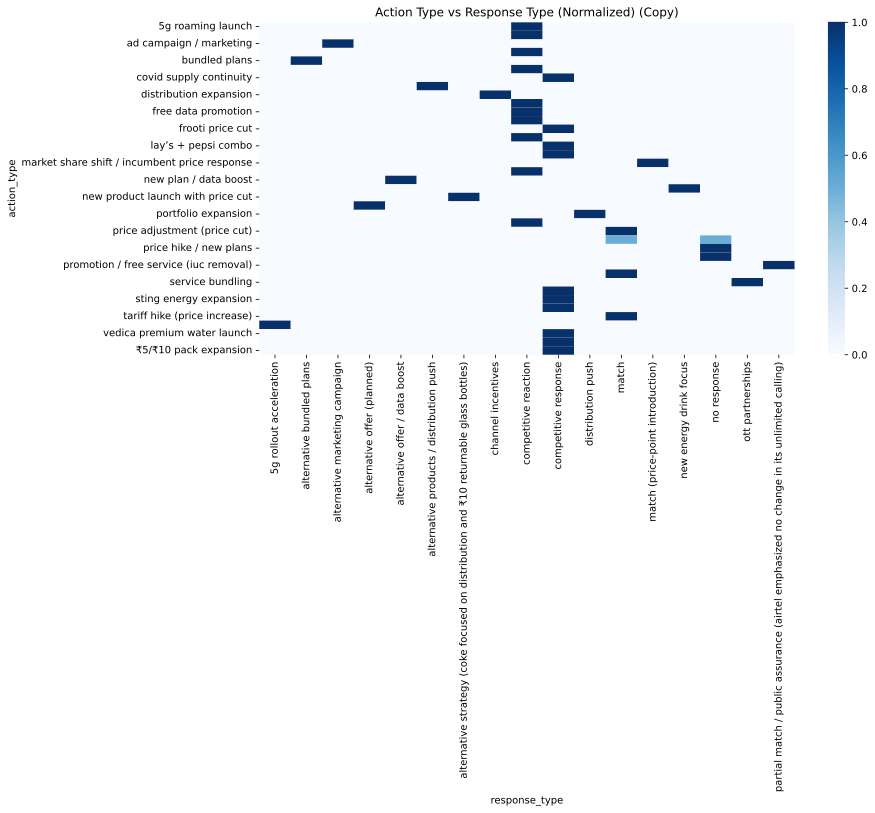
\includegraphics[width=0.8\textwidth]{figures/eda/action_type_vs_response_type_heatmap_copy.png}
    \caption{Action-Response Heatmap: Indian Telecom and FMCG. \textit{Interpretation:} Similar structure to Figure \ref{fig:heatmap}, but with more off-diagonal density. While price actions still trigger price responses (diagonal), we observe greater asymmetric behavior: price cuts met with alternative offers (data boosts, bundling) and product launches countered by distribution pushes rather than direct cloning. This reflects higher strategic flexibility in disruptive markets where firms possess asymmetric capabilities. The pattern supports the model assumption of differentiated payoff sensitivity, where capability constraints and cost heterogeneity make asymmetric responses rational.}
    \label{fig:heatmap_telecom}
\end{figure}

\subsubsection{When Asymmetry Is Rational}
\begin{itemize}
    \item \textbf{Cost heterogeneity:} A challenger may prefer product or channel moves if matching a rival's price is disproportionately costly.
    \item \textbf{Capability constraints:} Incumbents facing a disruptor may pivot to retention tools (bundles, service quality) rather than pure price matches.
    \item \textbf{Cycle alignment:} Firms exploit windows where rivals are committed to campaigns, choosing orthogonal moves that avoid direct margin erosion.
\end{itemize}

\subsection{Structural Drivers of Contrasts}
\begin{itemize}
    \item \textbf{Monitoring Technology and Observability:} Telecom tariffs are instantly observable; retail promotions are observable but with human-in-the-loop verification and store execution. Higher observability increases immediate retaliation and compresses lags \citep{Brynjolfsson2000}.
    \item \textbf{Adjustment Costs and Organizational Cadence:} Telecom has low menu costs for tariff changes, enabling 0-day responses. Retail/FMCG face higher adjustment costs for product/channel moves, producing longer tails \citep{Ferreira2021}.
    \item \textbf{Shock Sensitivity and Strategic Flexibility:} Crisis and policy shocks (COVID, inflation, regulation) push firms toward structural or product responses, elongating lags. Stable periods favor symmetric price matching within scheduled cycles.
\end{itemize}

\subsection{Economic Interpretation of EDA}
The high response rate and diagonal heatmap density are consistent with repeated-game enforcement: rapid matching nullifies unilateral gains, sustaining a low-margin equilibrium (the price-war trap) \citep{Ye2023}.
Telecom's 0-day spike implies near-perfect monitoring and high loss from delay, aligning with trigger strategies where deviations are punished immediately \citep{green1984noncooperative, Bichler2021}.
Longer lags in FMCG/product moves reflect adjustment costs and investment cycles; differentiation serves as a conditional escape from price wars when sufficiently valuable or defensible.

\section{Game Theoretic Framework}
Based on the empirical findings, we formulate a repeated non-cooperative game to model the observed dynamics \citep{Huang2024}.

\subsection{Model Setup}
Let $N = \{1, 2, ..., n\}$ be the set of players \citep{Chen2020}. We define the strategy space $S_i$ for player $i$ based on the observed actions:
\begin{equation}
    S_i = \{s_{\text{maintain}}, s_{\text{price}}, s_{\text{product}}, s_{\text{channel}}\}
\end{equation}
where $s_{\text{maintain}}$ represents the status quo, $s_{\text{price}}$ represents aggressive pricing or promotions, and $s_{\text{product}}/s_{\text{channel}}$ represent differentiation strategies \citep{hotelling1929stability}.

\subsection{Assumptions}
The model rests on four key assumptions derived from the EDA:
\begin{enumerate}
    \item \textbf{Imperfect Monitoring (Retail) vs. Perfect Visibility (Telecom)}: Justified by the difference in lag times (10 days vs. 0 days).
    \item \textbf{Deterministic Reaction Functions}: Justified by the strong diagonal density in the interaction heatmap.
    \item \textbf{Asymmetric Costs of Delay}: High churn risks in telecom force immediate responses.
    \item \textbf{Differentiated Payoff Sensitivity}: External shocks can alter the payoff matrix, favoring channel shifts \citep{Zhang2022}.
\end{enumerate}

\subsection{Payoff Structure}
We define an ordinal payoff matrix. Let $\pi_i(s_i, s_{-i})$ be the payoff for player $i$.
\begin{itemize}
    \item \textbf{Status Quo} $(0,0)$: Neutral market share.
    \item \textbf{Unilateral Aggression} $(G, -L)$: If Firm 1 cuts price ($s_p$) and Firm 2 maintains ($s_m$), Firm 1 gains share $G$ and Firm 2 loses $L$.
    \item \textbf{Price War} $(-C, -C)$: If both cut prices, share remains neutral, but margins erode.
    \item \textbf{Differentiation} $(V, V)$: If both differentiate ($s_d$), margins are preserved and value is created.
\end{itemize}

Table \ref{tab:payoff} presents the ordinal payoff matrix used in our analysis.

\begin{table}[H]
    \centering
    \caption{Ordinal Payoff Matrix}
    \label{tab:payoff}
    \begin{tabular}{l c c c}
        \toprule
        \textbf{P1 \textbackslash P2} & \textbf{Maintain ($s_m$)} & \textbf{Price Cut ($s_p$)} & \textbf{Product Diff ($s_d$)} \\
        \midrule
        \textbf{Maintain ($s_m$)} & $(0, 0)$ & $(-L, G)$ & $(-L, G)$ \\
        \textbf{Price Cut ($s_p$)} & $(G, -L)$ & $(-C, -C)$ & $(?, ?)$ \\
        \textbf{Product Diff ($s_d$)} & $(G, -L)$ & $(?, ?)$ & $(V, V)$ \\
        \bottomrule
    \end{tabular}
\end{table}

Figure \ref{fig:payoff} provides a visualization of this payoff landscape.

\begin{figure}[H]
    \centering
    \includegraphics[width=0.8\textwidth]{figures/game_theory/payoff_matrix.png}
    \caption{Payoff Matrix Visualization. \textit{Interpretation:} This heatmap represents the ordinal payoff structure for Player 1 (rows) and Player 2 (columns) across three strategies: Maintain status quo ($s_m$), Price Cut ($s_p$), and Product Differentiation ($s_d$). Cell colors indicate relative payoff values: red (negative/low), yellow (neutral), green (positive/high). The (Price Cut, Price Cut) cell shows mutual losses $(-C, -C)$—the price-war trap. Unilateral price cuts yield temporary gains $(G, -L)$, creating incentive for aggression. The (Differentiation, Differentiation) cell yields the highest mutual payoff $(V, V)$, representing the cooperative escape from margin erosion. This structure creates a Prisoner's Dilemma: price cutting is a dominant strategy in one-shot play, but mutual differentiation is Pareto-superior in repeated games with sufficient patience.}}
    \label{fig:payoff}
\end{figure}

\subsection{Player Sets}
Based on the EDA findings, we define two distinct player sets:
\begin{itemize}
    \item \textbf{Set A (Stable Duopoly):} $N_A = \{\text{Firm}_1, \text{Firm}_2\}$. Empirical Proxy: BIC Camera vs. Yodobashi Camera. Characteristics: High mutual monitoring, entrenched market positions.
    \item \textbf{Set B (Disruptive Oligopoly):} $N_B = \{\text{Incumbent}_1, \text{Incumbent}_2, \text{Disruptor}\}$. Empirical Proxy: Airtel/Vodafone vs. Reliance Jio; Coca-Cola vs. PepsiCo. Characteristics: Asymmetric capabilities, high-stakes market share battles.
\end{itemize}

\subsection{Game Type}
\subsubsection{Temporal Structure: Repeated Game}
The empirical evidence supports a repeated game formulation ($G^\infty$) \citep{maskin1988theory}. The response lag distribution shows continuous interaction cycles. Retail's consistent 7--14 day cycles imply a discrete time period $t$ (weekly), while Telecom's near-zero lag implies continuous time or very rapid $t$. The horizon is indefinite ($T \to \infty$).

\subsubsection{Nature of Play: Non-Cooperative}
The high response rate ($>90\%$) and the prevalence of price reductions and competitive reactions indicate a lack of collusion. Firms are actively defending market share rather than coordinating to maximize joint profits.

\subsection{Formal Game Theoretic Extensions}
\subsubsection{Strategy Formalization}
Let $h_t = (a^0, a^1, ..., a^{t-1})$ denote the public history. Given the EDA evidence of tit-for-tat (Retail) and immediate retaliation (Telecom), players utilize Markov strategies conditioned on the most recent $k$ states \citep{DenBoer2015}:
\begin{equation}
    \sigma_i(h_t) \approx \sigma_i(a_{-i, t-1}, ..., a_{-i, t-k})
\end{equation}
For Retail, $k \approx 7-14$ days. For Telecom, $k \to 0$ days.

\subsubsection{Payoff Function Decomposition}
We decompose the instantaneous payoff function $u_i(a)$ into Market Share Retention ($R$) and Profit Margin ($M$), adjusted by a differentiation parameter $\theta$:
\begin{equation}
    u_i(a_i, a_{-i}) = \alpha \cdot R(a_i, a_{-i}) + (1-\alpha) \cdot M(a_i) \cdot \mathbb{I}(a_i \neq a_{-i}) - C(a_i)
\end{equation}
where $\alpha \in [0,1]$ is the weight on market share, $\mathbb{I}(\cdot)$ is an indicator for product differentiation, and $C(a_i)$ is the implementation cost.

\subsubsection{Information Structure and Lag}
The Response Lag $\Delta_t$ acts as an information friction parameter.
\begin{itemize}
    \item \textbf{Perfect Monitoring (Telecom):} $\Delta_t \to 0$. Actions are observable immediately. This supports subgame-perfect equilibria with immediate punishment.
    \item \textbf{Imperfect Monitoring (Retail):} $\Delta_t \sim N(\mu=10, \sigma^2)$. Player $i$ observes a noisy signal $y_t$. This explains maintain periods where firms wait for confirmation before retaliating.
\end{itemize}

\subsection{Model Limitations}
\begin{enumerate}
    \item \textbf{Binary Response Simplification:} The model categorizes responses broadly, losing nuance in the magnitude of response (e.g., 5\% vs. 10\% price cut).
    \item \textbf{Lag Time Abstraction:} While we treat the game as repeated, the specific impact of the length of delay on the payoff function is not explicitly modeled, though EDA shows it varies by sector.
    \item \textbf{Missing Cost Data:} We assume cost structures based on margin implications, but lack direct financial data to quantify $C$ or $V$ precisely \citep{Elmaghraby2003}.
\end{enumerate}

\section{Equilibrium Analysis}
We analyze the game to identify stable outcomes.

\subsection{Static Nash Equilibrium}
In a one-shot game, the unique Nash equilibrium is $(s_{\text{price}}, s_{\text{price}})$. This is a classic Prisoner's Dilemma structure. If a rival plays $s_{\text{maintain}}$, the optimal response is $s_{\text{price}}$ to gain share ($G > 0$). If a rival plays $s_{\text{price}}$, the optimal response is $s_{\text{price}}$ to avoid the loss $L$ (assuming $-C > -L$). Thus, aggressive pricing is a dominant strategy.

\subsection{Dynamic Stability}
In the repeated game, the tit-for-tat strategy emerges as an enforcement mechanism. By credibly threatening to match any price cut immediately, firms reduce the expected gain from unilateral aggression \citep{Maskin2019}.
Figure \ref{fig:simulation} shows the simulation of strategies over time, illustrating how the system stabilizes in a low-payoff equilibrium or cycles through price wars.

\begin{figure}[H]
    \centering
    \includegraphics[width=0.8\textwidth]{figures/game_theory/repeated_game_simulation.png}
    \caption{Repeated Game Simulation Results. \textit{Interpretation:} The x-axis shows time periods (game rounds), and the y-axis tracks cumulative payoffs for two players. The simulation demonstrates how tit-for-tat strategies stabilize in repeated play: after initial experimentation, both players settle into a pattern of mutual maintenance punctuated by occasional defensive matching. The convergence to a low-variance payoff trajectory illustrates the Red Queen effect—firms run fast just to stay in place. Divergence events (payoff gaps) occur when one player attempts differentiation, which either succeeds (sustained gap) or triggers retaliation (convergence). This validates the empirical observation that 90\%+ of actions elicit responses, supporting equilibrium stability through threat credibility.}
    \label{fig:simulation}
\end{figure}

\subsection{Stability Analysis and Robustness}
\subsubsection{Robustness to Trembles}
In the empirical context, trembles correspond to accidental price changes or misinterpretation of rival moves.
For the Retail Sector, with imperfect monitoring ($\Delta_t > 0$), a Grim Trigger is fragile. Stability requires firms to utilize Green-Porter style trigger phases where punishment lasts for $T$ periods rather than infinity.

\subsubsection{Renegotiation Proofness}
Once a punishment phase $(-C, -C)$ begins, both firms have an incentive to renegotiate. The existence of differentiation ($s_d$) offers a Pareto-improving exit path. The equilibrium is weakly renegotiation-proof if firms can coordinate on switching to $s_d$ (Product Innovation) rather than simply reverting to $s_m$.

\subsection{Comparative Statics}
\subsubsection{Impact of Response Lag ($\Delta_t$)}
As $\Delta_t$ decreases (faster detection), the gain from defection shrinks and punishment arrives sooner. Thus, faster monitoring (Telecom) makes cooperation easier to sustain in theory, or punishment swifter if broken.

\subsubsection{Impact of Differentiation ($\theta$)}
Higher differentiation increases the cooperative payoff $V$. This lowers the critical discount factor $\delta^*$, expanding the set of parameters where peace is stable. This explains why FMCG sees fewer pure price wars than Telecom.

\subsection{Industry-Specific Equilibrium Cases}
\subsubsection{Case A: Japanese Electronics Retail}
With $\Delta_t \approx 10$ days and high product homogeneity, the equilibrium is a risk-dominant coordinate. Firms are in a coordination game where matching is safer than leading. The tit-for-tat discipline enforces stable cycles of promotion and matching.

\subsubsection{Case B: Indian Telecom}
With $\Delta_t \approx 0$ and high market share focus, the equilibrium is an aggressive Nash equilibrium. If the goal is market exit of a rival, the game becomes a war of attrition, leading to intense, low-margin equilibrium until market consolidation.

\subsection{Economic Interpretation of Equilibrium}
\begin{itemize}
    \item \textbf{Efficiency and Welfare:} The price cut equilibrium maximizes consumer surplus in the short run but harms producer surplus.
    \item \textbf{The Red Queen Effect:} Firms must constantly respond just to maintain share. In Retail, this is promotional churn; in Telecom, feature escalation.
    \item \textbf{Strategic Recommendation:} To escape the low-profit trap, firms must increase differentiation to decouple reaction functions.
\end{itemize}

\section{Results and Discussion}
The model provides a robust explanation for the observed market behaviors.

\subsection{Predictive Power}
The model correctly predicts the high response rate observed in the data. The prediction that no response is an unstable outcome aligns with the empirical finding that it occurs in only 7.5\% of cases. The dominance of price matching in the electronics sector confirms the static Nash equilibrium prediction.

\subsection{Escape Strategies}
The only conditional escape from the price trap is product differentiation. In the FMCG sector, we observed firms responding to price pressure with new product launches. This effectively shifts the game to the $(s_{\text{product}}, s_{\text{product}})$ cell, where payoffs are $(V, V)$. This aligns with \cite{porter1980competitive} theories on differentiation strategies.

\subsection{Interpretation of Dominant Strategies}
Price cutting emerges as a dominant strategy because it offers protection against being undercut (defensive) and yields share gain if the rival maintains (offensive). Differentiation is a conditional strategy, yielding high returns only when matched or sufficiently unique.

\subsection{Theoretical Connections}
\begin{itemize}
    \item \textbf{Tacit Collusion and Green-Porter (1984):} The maintain phases punctuated by price matching in Retail align with Green and Porter's model of non-cooperative collusion under imperfect information.
    \item \textbf{Maskin and Tirole (1988):} The deterministic nature of responses supports Markov Perfect Equilibria, where strategies depend only on the payoff-relevant state.
    \item \textbf{Hotelling (1929):} The divergence between price and channel strategies reflects the principle of minimum vs. maximal differentiation.
    \item \textbf{Porter's Strategic Groups:} The separation of stable duopoly and disruptive oligopoly validates Porter's theory, implying mobility barriers prevent retail logic from applying to telecom \citep{Zhao2020}.
\end{itemize}

\section{Strategic Implications and Policy Recommendations}

\subsection{Managerial Implications}
\subsubsection{The Red Queen Trap and Strategic Exit}
Firms in high-response environments often fall into a Red Queen effect. Managers should audit their response portfolio. If the majority of actions are purely defensive price matches, the firm is in a value-destroying equilibrium. A strategic pivot from reaction speed to differentiation latency is recommended.

\subsubsection{Managing the Signal-to-Noise Ratio}
In Retail, increasing the complexity of promotions can dampen the tit-for-tat response. In Telecom, credible commitments (e.g., price match guarantee) can soften competition.

\subsubsection{Asymmetric Response Framework}
Incumbents facing a disruptor should avoid symmetric price wars. Instead of matching price, they should match value or change the metric (e.g., compete on network reliability).

\subsection{Policy Considerations}
\begin{itemize}
    \item \textbf{Algorithmic Collusion Risks:} Instantaneous, deterministic matching is a marker for algorithmic coordination. Regulators should monitor response latency \citep{Ezrachi2019, Harrington2018}.
    \item \textbf{Predatory Pricing:} If a price war persists while investment drops, intervention may be required \citep{Jena2025}.
    \item \textbf{Consumer Welfare Paradox:} Policy should balance immediate price benefits with the health of the innovation ecosystem to avoid commoditization traps \citep{Klein2022}.
\end{itemize}

\subsection{Cross-Industry Structural Drivers}
Retail behaves like a repeated partnership, where maintaining the status quo is mutually beneficial. Telecom behaves like a war of attrition, motivating high burn rates to outlast opponents.

\section{Conclusion and Future Work}
We have demonstrated that aggressive pricing is a dominant defensive strategy in oligopolistic markets, confirmed by both EDA and game-theoretic modeling. The tit-for-tat dynamic, while preventing unilateral dominance, often traps firms in a cycle of margin erosion.

\textbf{Limitations:} Our model relies on binary response simplifications and lacks precise internal cost data ($C$ vs. $L$). Future work could incorporate asymmetric information and regulatory interventions to refine the payoff functions.

\bibliographystyle{apalike}
\bibliography{references}

\end{document}
